\documentclass[11pt]{article}
\usepackage[a4paper,margin=1in]{geometry}
\usepackage[T1]{fontenc}
\usepackage[utf8]{inputenc}
\usepackage{lmodern}
\usepackage{amsmath}
\usepackage{booktabs}
\usepackage{hyperref}
\usepackage{tikz}
\usetikzlibrary{arrows.meta,positioning,shapes.geometric,shapes.misc,fit,calc}

\title{Pixiv Downloader Workflow and Data Structures}
\author{pixiv\_downloader Project Notes}
\date{\today}

\begin{document}
\maketitle

\section{Purpose}
This document explains:
\begin{enumerate}
    \item The current end-to-end workflow of the downloader.
    \item How data is stored on disk.
    \item Which data structures are used and why.
    \item Time and space complexity of major operations.
    \item How an offline local viewer uses local metadata/images only.
\end{enumerate}

\paragraph{Complexity Symbols}
\begin{itemize}
    \item $K$: number of search keywords.
    \item $P$: max pages requested per keyword.
    \item $R$: average results per search page.
    \item $A$: accepted artworks after filtering.
    \item $U$: total image URLs across accepted artworks.
    \item $T$: average tag count per artwork.
    \item $M$: artworks with missing likes that need detail backfill.
\end{itemize}

\section{Workflow Overview}
\subsection{Main Stages}
\begin{enumerate}
    \item Parse runtime options and normalize filters.
    \item Branch by mode:
    \begin{itemize}
        \item \texttt{first\_download=True}: start with empty metadata map.
        \item \texttt{first\_download=False}: load existing \texttt{tags.json}.
    \end{itemize}
    \item Build download plan from search API pages.
    \item Expand each planned artwork into original image URLs.
    \item Download files (serial or thread pool).
    \item Backfill missing likes metadata if needed.
    \item Persist metadata and indexes atomically.
    \item Write run report text file.
\end{enumerate}

\begin{figure}[htbp]
\centering
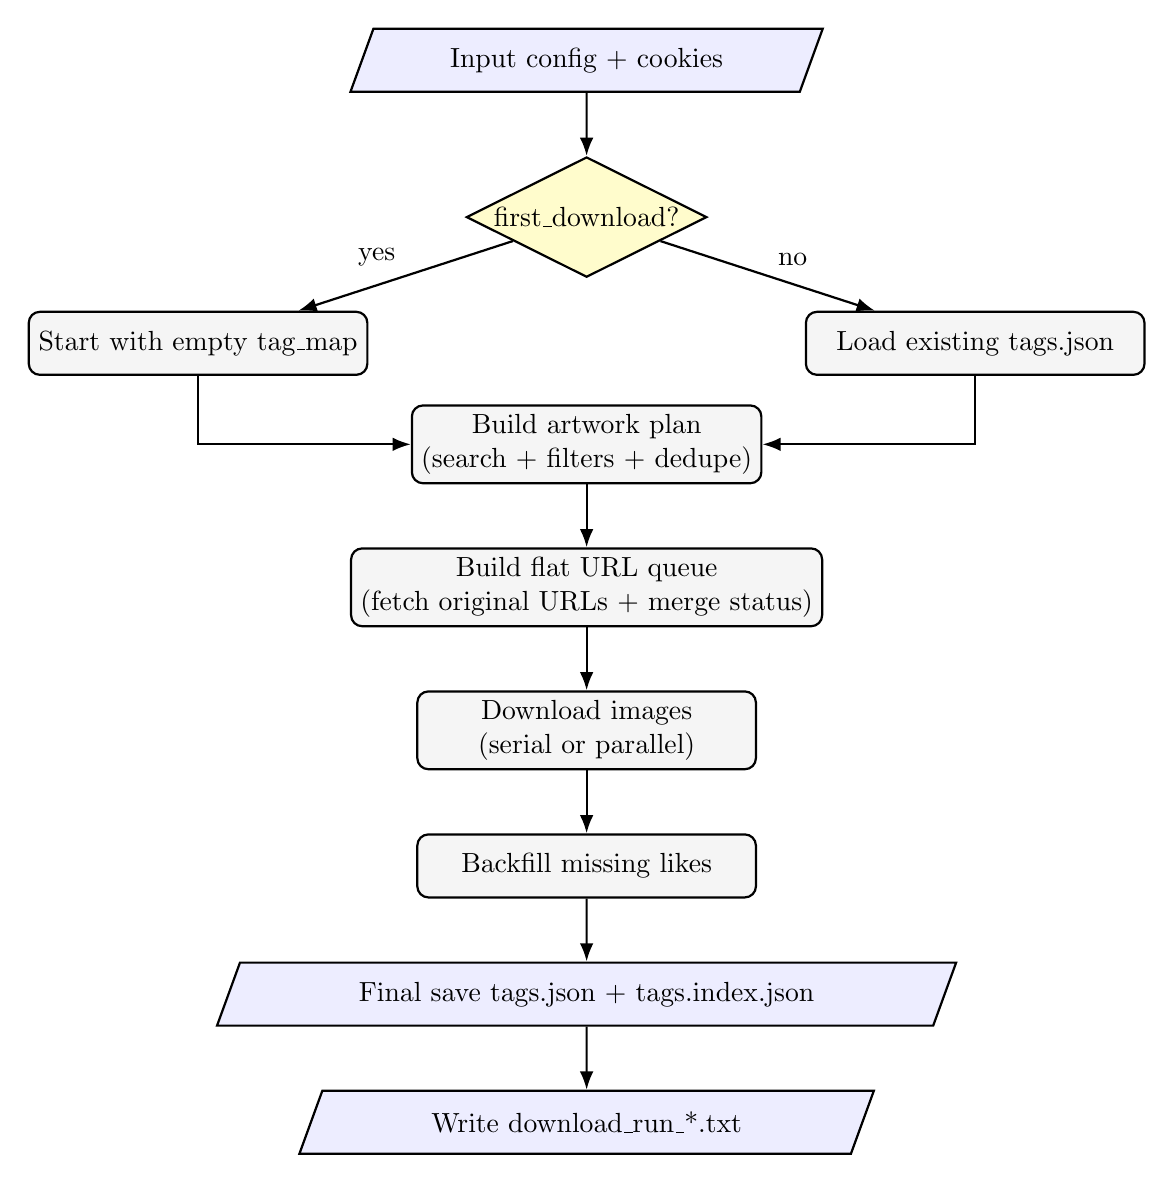
\begin{tikzpicture}[
    node distance=8mm and 12mm,
    block/.style={rectangle, rounded corners, draw=black, thick, align=center, minimum width=4.3cm, minimum height=8mm, fill=gray!8},
    decision/.style={diamond, draw=black, thick, aspect=2, align=center, inner sep=1pt, fill=yellow!20},
    io/.style={trapezium, trapezium left angle=70, trapezium right angle=110, draw=black, thick, align=center, minimum width=3.9cm, minimum height=8mm, fill=blue!7},
    line/.style={-Latex, thick}
]
\node[io] (start) {Input config + cookies};
\node[decision, below=of start] (mode) {first\_download?};
\node[block, below left=of mode, xshift=-8mm] (fresh) {Start with empty tag\_map};
\node[block, below right=of mode, xshift=8mm] (inc) {Load existing tags.json};
\node[block, below=16mm of mode] (plan) {Build artwork plan\\(search + filters + dedupe)};
\node[block, below=of plan] (queue) {Build flat URL queue\\(fetch original URLs + merge status)};
\node[block, below=of queue] (download) {Download images\\(serial or parallel)};
\node[block, below=of download] (likes) {Backfill missing likes};
\node[io, below=of likes] (persist) {Final save tags.json + tags.index.json};
\node[io, below=of persist] (report) {Write download\_run\_*.txt};

\draw[line] (start) -- (mode);
\draw[line] (mode) -- node[above left]{yes} (fresh);
\draw[line] (mode) -- node[above right]{no} (inc);
\draw[line] (fresh) |- (plan);
\draw[line] (inc) |- (plan);
\draw[line] (plan) -- (queue);
\draw[line] (queue) -- (download);
\draw[line] (download) -- (likes);
\draw[line] (likes) -- (persist);
\draw[line] (persist) -- (report);
\end{tikzpicture}
\caption{Current downloader pipeline.}
\end{figure}

\paragraph{Checkpoint Write Policy}
In incremental mode, metadata refresh and likes backfill may write checkpoint updates to \texttt{tags.json}.
In first-download mode, likes backfill updates remain in memory and are persisted at final save.

\section{Data Storage Layout}
\subsection{Image Files}
Downloaded images are stored in the destination folder using filenames derived from the Pixiv original URL basename.

\subsection{Metadata File}
Metadata is stored in \texttt{tags.json} under the destination folder.

\paragraph{Example shape}
\begin{verbatim}
{
  "<artwork_id>": {
        "artwork_id": "...",
    "author_id": 123456,
    "author_name": "...",
    "post_date": "YYYY-MM-DD",
    "likes": 999,
        "tags": ["tag_a", "tag_b"],
        "local_files": ["123_p0.jpg", "123_p1.jpg"],
        "url_status": "ok|url_not_found|forbidden|request_error",
        "download_status": "downloaded|partial|download_failed|url_not_found",
        "first_seen_at": "ISO8601",
        "last_refreshed_at": "ISO8601",
        "last_download_at": "ISO8601"
  }
}
\end{verbatim}

\subsection{Sort Index File}
Sort indexes are stored in \texttt{tags.index.json} and contain precomputed id lists for:
\begin{itemize}
        \item \texttt{likes} (asc/desc)
        \item \texttt{post\_date} (asc/desc)
        \item \texttt{artwork\_id} (asc/desc)
\end{itemize}

\subsection{Run Report File}
Each run writes \texttt{download\_run\_YYYYMMDD\_HHMMSS\_mmmmmm.txt}. If a collision occurs, suffixes
such as \texttt{\_1}, \texttt{\_2} are appended.

\subsection{Atomic Write Behavior}
JSON persistence writes to a unique temp file first and then calls \texttt{os.replace}. On Windows,
replace is retried briefly on transient \texttt{PermissionError} to reduce file lock failures.

\section{Data Structures in Code}
\begin{itemize}
    \item \textbf{seen} (set): deduplicate artwork ids during planning.
    \item \textbf{planned\_artworks} (list of dict): accepted artwork metadata before URL expansion.
    \item \textbf{tag\_map} (dict): runtime metadata map keyed by artwork id.
    \item \textbf{download\_tasks} (list of dict): flat file-level queue for downloads.
    \item \textbf{artwork\_with\_urls} (set): artworks whose original URLs were resolved.
    \item \textbf{successful\_pids} (set): artworks with at least one successful file write.
    \item \textbf{refreshed\_pids} / \textbf{new\_artwork\_ids} (set): track refresh/new status by mode.
    \item \textbf{expected\_files\_by\_pid} / \textbf{downloaded\_files\_by\_pid} (dict): compute precise download status.
    \item \textbf{thread-local session} (\texttt{threading.local}): one HTTP session per worker thread.
\end{itemize}

\begin{figure}[htbp]
\centering
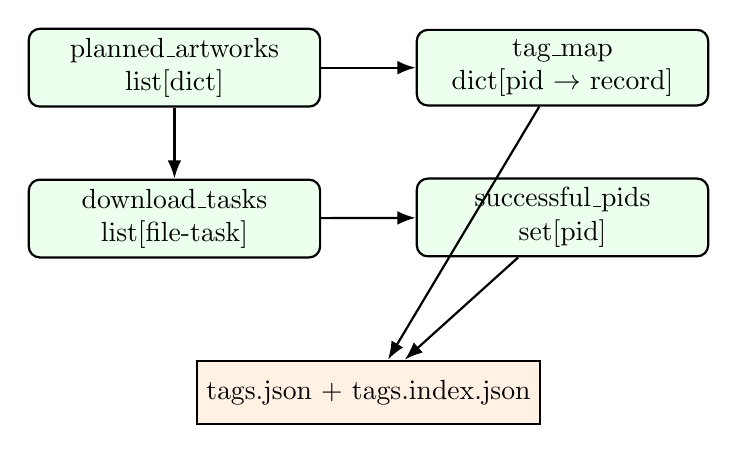
\begin{tikzpicture}[
    node distance=9mm and 12mm,
    ds/.style={rectangle, draw=black, thick, rounded corners, align=center, minimum width=3.7cm, minimum height=8mm, fill=green!7},
    file/.style={rectangle, draw=black, thick, align=center, minimum width=3.7cm, minimum height=8mm, fill=orange!10},
    arr/.style={-Latex, thick}
]
\node[ds] (plan) {planned\_artworks\\ list[dict]};
\node[ds, right=of plan] (meta) {tag\_map\\ dict[pid $\to$ record]};
\node[ds, below=of plan] (queue) {download\_tasks\\ list[file-task]};
\node[ds, below=of meta] (succ) {successful\_pids\\ set[pid]};
\node[file, below=18mm of $(queue)!0.5!(succ)$] (json) {tags.json + tags.index.json};

\draw[arr] (plan) -- (meta);
\draw[arr] (plan) -- (queue);
\draw[arr] (queue) -- (succ);
\draw[arr] (meta) -- (json);
\draw[arr] (succ) -- (json);
\end{tikzpicture}
\caption{Core runtime structures and metadata output path.}
\end{figure}

\section{Complexity Summary}
\subsection{Stage Complexity}
\begin{itemize}
    \item \textbf{Plan build}: inspect approximately $K \cdot P \cdot R$ search items, with tag checks around $O(T)$ each. Practical bound $O(KPRT)$.
    \item \textbf{URL expansion}: one pages-endpoint call per accepted artwork plus flattening all URLs, around $O(A + U)$ plus network latency.
    \item \textbf{Download stage}: one request per URL, around $O(U)$ request operations.
    \item \textbf{Likes backfill}: up to $M$ detail calls, around $O(M)$ plus network latency.
    \item \textbf{Metadata write}: linear in output metadata size.
    \item \textbf{Sort index build}: approximately $O(N \log N)$ per sort key.
\end{itemize}

\subsection{Space Complexity}
Dominant memory terms:
\[
O(A + U)
\]
where $A$ is artwork-level plan size and $U$ is flat file queue size.

\begin{table}[htbp]
\centering
\begin{tabular}{@{}lll@{}}
\toprule
Structure & Typical Operation & Average Complexity \\
\midrule
set (seen, success ids) & membership/add & $O(1)$ \\
dict (metadata map) & get/set by id & $O(1)$ \\
list (planned queue) & append & amortized $O(1)$ \\
list (download tasks) & append/iterate & amortized $O(1)$ / $O(U)$ \\
thread pool futures & collect completed tasks & $O(U)$ overall \\
\bottomrule
\end{tabular}
\caption{Operation complexity by structure.}
\end{table}

\section{Offline Local Viewer Concept}
A small local viewer can run without internet by reading only:
\begin{enumerate}
    \item local image files,
    \item \texttt{tags.json} metadata,
    \item \texttt{tags.index.json} sort indexes (if available).
\end{enumerate}

Suggested in-memory indexes:
\begin{itemize}
    \item \textbf{artwork\_by\_id}: dict for direct lookup.
    \item \textbf{tag\_to\_ids}: inverted index for fast tag filtering.
    \item \textbf{sorted id lists}: loaded from persisted sort index file.
    \item \textbf{current ordered ids}: result sequence after filter+sort for table/gallery/lightbox.
\end{itemize}

\begin{figure}[htbp]
\centering
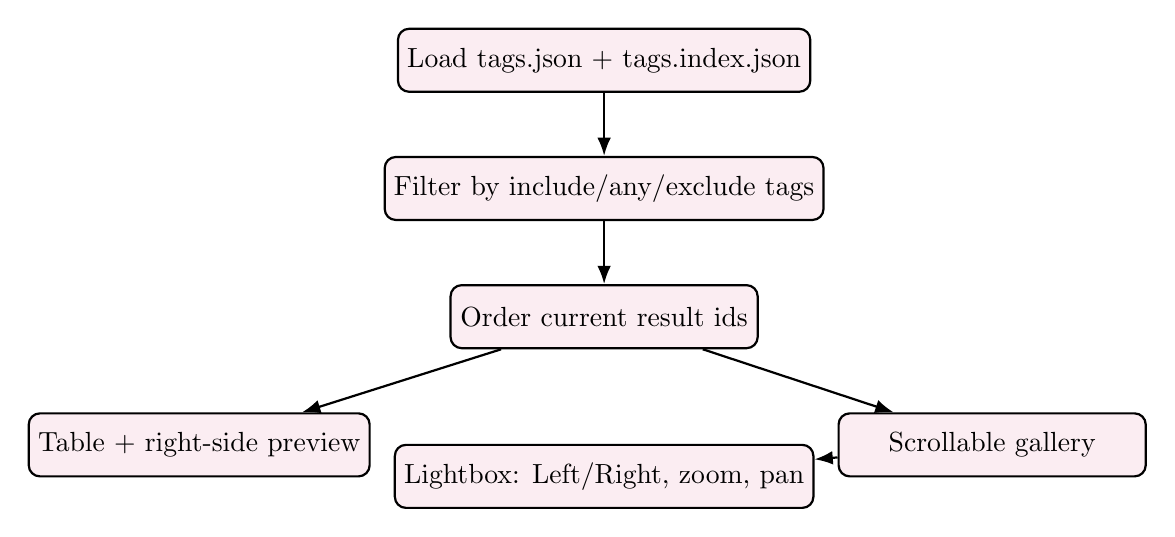
\begin{tikzpicture}[
    node distance=8mm and 10mm,
    box/.style={rectangle, draw=black, thick, rounded corners, minimum width=3.9cm, minimum height=8mm, align=center, fill=purple!7},
    arr/.style={-Latex, thick}
]
\node[box] (load) {Load tags.json + tags.index.json};
\node[box, below=of load] (filter) {Filter by include/any/exclude tags};
\node[box, below=of filter] (order) {Order current result ids};
\node[box, below left=of order] (table) {Table + right-side preview};
\node[box, below right=of order] (gallery) {Scrollable gallery};
\node[box, below=12mm of order] (lightbox) {Lightbox: Left/Right, zoom, pan};

\draw[arr] (load) -- (filter);
\draw[arr] (filter) -- (order);
\draw[arr] (order) -- (table);
\draw[arr] (order) -- (gallery);
\draw[arr] (gallery) -- (lightbox);
\end{tikzpicture}
\caption{Offline viewer flow based on local metadata and files only.}
\end{figure}

\section{Build Notes}
Compile with a LaTeX engine that supports TikZ, for example:
\begin{verbatim}
pdflatex downloader_workflow_and_data_structures.tex
\end{verbatim}

\end{document}
